% Options for packages loaded elsewhere
\PassOptionsToPackage{unicode}{hyperref}
\PassOptionsToPackage{hyphens}{url}
\PassOptionsToPackage{dvipsnames,svgnames,x11names}{xcolor}
%
\documentclass[
  12pt,
  letterpaper,
  DIV=11,
  numbers=noendperiod]{scrartcl}

\usepackage{amsmath,amssymb}
\usepackage{iftex}
\ifPDFTeX
  \usepackage[T1]{fontenc}
  \usepackage[utf8]{inputenc}
  \usepackage{textcomp} % provide euro and other symbols
\else % if luatex or xetex
  \usepackage{unicode-math}
  \defaultfontfeatures{Scale=MatchLowercase}
  \defaultfontfeatures[\rmfamily]{Ligatures=TeX,Scale=1}
\fi
\usepackage{lmodern}
\ifPDFTeX\else  
    % xetex/luatex font selection
\fi
% Use upquote if available, for straight quotes in verbatim environments
\IfFileExists{upquote.sty}{\usepackage{upquote}}{}
\IfFileExists{microtype.sty}{% use microtype if available
  \usepackage[]{microtype}
  \UseMicrotypeSet[protrusion]{basicmath} % disable protrusion for tt fonts
}{}
\makeatletter
\@ifundefined{KOMAClassName}{% if non-KOMA class
  \IfFileExists{parskip.sty}{%
    \usepackage{parskip}
  }{% else
    \setlength{\parindent}{0pt}
    \setlength{\parskip}{6pt plus 2pt minus 1pt}}
}{% if KOMA class
  \KOMAoptions{parskip=half}}
\makeatother
\usepackage{xcolor}
\usepackage[margin=1in]{geometry}
\setlength{\emergencystretch}{3em} % prevent overfull lines
\setcounter{secnumdepth}{-\maxdimen} % remove section numbering
% Make \paragraph and \subparagraph free-standing
\ifx\paragraph\undefined\else
  \let\oldparagraph\paragraph
  \renewcommand{\paragraph}[1]{\oldparagraph{#1}\mbox{}}
\fi
\ifx\subparagraph\undefined\else
  \let\oldsubparagraph\subparagraph
  \renewcommand{\subparagraph}[1]{\oldsubparagraph{#1}\mbox{}}
\fi


\providecommand{\tightlist}{%
  \setlength{\itemsep}{0pt}\setlength{\parskip}{0pt}}\usepackage{longtable,booktabs,array}
\usepackage{calc} % for calculating minipage widths
% Correct order of tables after \paragraph or \subparagraph
\usepackage{etoolbox}
\makeatletter
\patchcmd\longtable{\par}{\if@noskipsec\mbox{}\fi\par}{}{}
\makeatother
% Allow footnotes in longtable head/foot
\IfFileExists{footnotehyper.sty}{\usepackage{footnotehyper}}{\usepackage{footnote}}
\makesavenoteenv{longtable}
\usepackage{graphicx}
\makeatletter
\def\maxwidth{\ifdim\Gin@nat@width>\linewidth\linewidth\else\Gin@nat@width\fi}
\def\maxheight{\ifdim\Gin@nat@height>\textheight\textheight\else\Gin@nat@height\fi}
\makeatother
% Scale images if necessary, so that they will not overflow the page
% margins by default, and it is still possible to overwrite the defaults
% using explicit options in \includegraphics[width, height, ...]{}
\setkeys{Gin}{width=\maxwidth,height=\maxheight,keepaspectratio}
% Set default figure placement to htbp
\makeatletter
\def\fps@figure{htbp}
\makeatother
\newlength{\cslhangindent}
\setlength{\cslhangindent}{1.5em}
\newlength{\csllabelwidth}
\setlength{\csllabelwidth}{3em}
\newlength{\cslentryspacingunit} % times entry-spacing
\setlength{\cslentryspacingunit}{\parskip}
\newenvironment{CSLReferences}[2] % #1 hanging-ident, #2 entry spacing
 {% don't indent paragraphs
  \setlength{\parindent}{0pt}
  % turn on hanging indent if param 1 is 1
  \ifodd #1
  \let\oldpar\par
  \def\par{\hangindent=\cslhangindent\oldpar}
  \fi
  % set entry spacing
  \setlength{\parskip}{#2\cslentryspacingunit}
 }%
 {}
\usepackage{calc}
\newcommand{\CSLBlock}[1]{#1\hfill\break}
\newcommand{\CSLLeftMargin}[1]{\parbox[t]{\csllabelwidth}{#1}}
\newcommand{\CSLRightInline}[1]{\parbox[t]{\linewidth - \csllabelwidth}{#1}\break}
\newcommand{\CSLIndent}[1]{\hspace{\cslhangindent}#1}

\usepackage[default]{sourcesanspro}
\usepackage{sourcecodepro}
\usepackage{lineno}
\linenumbers
\linespread{1.2}
\KOMAoption{captions}{tableheading}
\makeatletter
\makeatother
\makeatletter
\makeatother
\makeatletter
\@ifpackageloaded{caption}{}{\usepackage{caption}}
\AtBeginDocument{%
\ifdefined\contentsname
  \renewcommand*\contentsname{Table of contents}
\else
  \newcommand\contentsname{Table of contents}
\fi
\ifdefined\listfigurename
  \renewcommand*\listfigurename{List of Figures}
\else
  \newcommand\listfigurename{List of Figures}
\fi
\ifdefined\listtablename
  \renewcommand*\listtablename{List of Tables}
\else
  \newcommand\listtablename{List of Tables}
\fi
\ifdefined\figurename
  \renewcommand*\figurename{Fig.}
\else
  \newcommand\figurename{Fig.}
\fi
\ifdefined\tablename
  \renewcommand*\tablename{Table}
\else
  \newcommand\tablename{Table}
\fi
}
\@ifpackageloaded{float}{}{\usepackage{float}}
\floatstyle{ruled}
\@ifundefined{c@chapter}{\newfloat{codelisting}{h}{lop}}{\newfloat{codelisting}{h}{lop}[chapter]}
\floatname{codelisting}{Listing}
\newcommand*\listoflistings{\listof{codelisting}{List of Listings}}
\makeatother
\makeatletter
\@ifpackageloaded{caption}{}{\usepackage{caption}}
\@ifpackageloaded{subcaption}{}{\usepackage{subcaption}}
\makeatother
\makeatletter
\@ifpackageloaded{tcolorbox}{}{\usepackage[skins,breakable]{tcolorbox}}
\makeatother
\makeatletter
\@ifundefined{shadecolor}{\definecolor{shadecolor}{rgb}{.97, .97, .97}}
\makeatother
\makeatletter
\makeatother
\makeatletter
\makeatother
\ifLuaTeX
  \usepackage{selnolig}  % disable illegal ligatures
\fi
\IfFileExists{bookmark.sty}{\usepackage{bookmark}}{\usepackage{hyperref}}
\IfFileExists{xurl.sty}{\usepackage{xurl}}{} % add URL line breaks if available
\urlstyle{same} % disable monospaced font for URLs
\hypersetup{
  colorlinks=true,
  linkcolor={blue},
  filecolor={Maroon},
  citecolor={Blue},
  urlcolor={Blue},
  pdfcreator={LaTeX via pandoc}}

\author{}
\date{}

\begin{document}
\ifdefined\Shaded\renewenvironment{Shaded}{\begin{tcolorbox}[sharp corners, boxrule=0pt, interior hidden, borderline west={3pt}{0pt}{shadecolor}, enhanced, frame hidden, breakable]}{\end{tcolorbox}}\fi

\newpage

\textbf{The effect of artificial light at night (ALAN) on understory
plants: an experiment in a rubber plantation in China}

\[ \]

Cong Zhou\textsuperscript{1,2}, Akihiro Nakamura\textsuperscript{1},
Xiaoyang Song\textsuperscript{1}, Masatoshi Katabuchi\textsuperscript{1}

\[ \]

\textsuperscript{1} CAS Key Laboratory of Tropical Forest Ecology,
Xishuangbanna Tropical Botanical Garden, Chinese Academy of Sciences,
Menglun, Yunnan 666303, China

\textsuperscript{2} University of Chinese Academy of Sciences, Beijing
100049, China

\[ \]

\textbf{Corresponding Authors}:

Masatoshi Katabuchi

E-mail: katabuchi@xtbg.ac.cn; mattocci27@gmail.com

\[ \]

\textbf{Running title}:

\newpage

\hypertarget{abstract}{%
\section{ABSTRACT}\label{abstract}}

Artificial light at night (ALAN) demonstrated a new ecological factor
that influences organisms through multi-approach. As yet, assessing the
impacts of artificial light at night on understory plants has little
attention. We evaluated whether ALAN would affect the LMA (leaf mass per
area) of understory plants through a two-year field light experiment in
a tropical rubber plantation in south China. We hypothesized that ALAN
could impact the understory in two ways: by directly supplementing light
to aboveground plant parts and indirectly by attracting insects, which
could alter soil nutrient composition underground. We selected two
species: \emph{Colocasia gigantea}, representing shade species and
\emph{Melastoma candidum}, representing sun species. We measured canopy
openness, LMA, soil nutrients and individual distance away from ALAN. We
found a negative relationship between LMA and the effects of ALAN. This
relationship was significant for \emph{Colocasia gigantea} but not for
\emph{Melastoma candidum}. These results suggest that ALAN might have
complex and multifaceted impacts on the understory ecosystem.

\textbf{KEY WORDS} \emph{Colocasia gigantea}, \emph{Melastoma candidum},
artificial light at night, functional traits, leaf mass per area,
specific leaf area, understory

\hypertarget{introduction}{%
\section{INTRODUCTION}\label{introduction}}

Artificial light at night (ALAN), a leading contributor to light
pollution, has disrupted ecological processes since the early 20th
century (\protect\hyperlink{ref-Longcore2004}{Longcore and Rich 2004},
\protect\hyperlink{ref-Gaston2013}{Gaston et al. 2013},
\protect\hyperlink{ref-Bennie2016}{Bennie et al. 2016}). A recent study
estimated that around 23\% of the world's inhabited land surfaces,
accounting for over 80\% of the global population, are subject to the
adverse effects of light pollution
(\protect\hyperlink{ref-Falchi2016}{2016}). Although the intensity of
ALAN varies several orders of magnitude from faint skyglow reflected
from distant cities to direct illumination of urban and suburban
vegetation (\protect\hyperlink{ref-Bennie2016}{Bennie et al. 2016}),
ALAN could influence the behaviour or physiology of broad ranges of
taxonomic groups, including mammals, birds, reptiles, amphibians,
fishes, invertebrates, and plants. It could alter ecosystem functions
(\protect\hyperlink{ref-Rich2006}{Rich and Longcore 2006}). For example,
ALAN attracts insects interfering in movement, foraging, reproduction,
and development, as an important bringer to driving insect population
decline (\protect\hyperlink{ref-Owens2020}{Owens et al. 2020},
\protect\hyperlink{ref-Boyes2021}{Boyes et al. 2021}). Many studies have
focused on how ALAN changes the behaviour of animals
(\protect\hyperlink{ref-Russart2018}{Russart and Nelson 2018}). However,
only a handful of studies have been published on the effect of ALAN on
plants (\protect\hyperlink{ref-Bennie2016}{Bennie et al. 2016},
\protect\hyperlink{ref-Speisser2021a}{Speißer et al. 2021},
\protect\hyperlink{ref-Liu2022}{Liu et al. 2022}). Speißer et al.
(\protect\hyperlink{ref-Speisser2021a}{2021}) conducted plant growth
experiments with and without weak ALAN (28 lx: within the range of light
intensities at ground level under street lights) and showed that ALAN
increases the biomass of herbaceous plants. Their results suggest that
even weak ALAN acts as a light resource for plant growth. However, few
studies have examined the effects of ALAN on plant functional traits in
conditions close to their natural environment.

ALAN might, directly and indirectly, affect plant leaf functional
traits. First, ALAN might directly affect plant leaf functional traits
because ALAN could work as a light resource. Although LMA is driven by
inherent genetic mechanisms (\protect\hyperlink{ref-Asner2011}{Asner et
al. 2011}), environmental stresses (temperature, water and light) also
shape LMA. Plants can sense light through photoreceptors, allowing them
to respond to four parameters of their light environment: light spectral
quality, light intensity, light direction, and light duration
(\protect\hyperlink{ref-Rich2006}{Rich and Longcore 2006},
\protect\hyperlink{ref-Paik2019}{Paik and Huq 2019}). Terashima et al.
(\protect\hyperlink{ref-Terashima2006}{2006}) showed that the
light-saturated rate of leaf photosynthesis per unit area is highly
correlated with leaf structural parameters such as leaf thickness, leaf
mass per area, mesophyll surface area, and chloroplast surface area, and
sun leaves are thicker than shade leaves as the height of the palisade
tissue in sun leaves is greater than that in shade leaves. For
individual species, LMA was proportional with species distributions
along the insolation gradient and was significantly higher in evergreen
versus deciduous species (\protect\hyperlink{ref-Ackerly2002}{Ackerly et
al. 2002}, \protect\hyperlink{ref-Niinemets2004}{Niinemets et al. 2004},
\protect\hyperlink{ref-Onoda2008}{Onoda et al. 2008}). Moreover, among a
local community, Ackerly et al.
(\protect\hyperlink{ref-Ackerly2002}{2002}) demonstrated that the
average values of LMA significantly increased with increasing potential
diurnal insolation (PDI).

On the other hand, ALAN might indirectly affect plant leaf functional
traits because ALAN has the potential to change soil fertility by
attracting insects. Many insects orient themselves by maintaining a
constant angle to light rays and are attracted by light
(\protect\hyperlink{ref-Baker1978}{Baker and Sadovy 1978},
\protect\hyperlink{ref-Sotthibandhu1979}{Sotthibandhu and Baker 1979}).
Previous studies showed that 30--40\% of insects die soon after
approaching street lamps for collision, overheating, dehydration, or
predation (\protect\hyperlink{ref-Minnaar2015}{Minnaar et al. 2015},
\protect\hyperlink{ref-Owens2018}{Owens and Lewis 2018}). Since nitrogen
(N) and phosphorus (P) are the nutrients most frequently limiting
primary productivity in forest ecosystems
(\protect\hyperlink{ref-Wright2019}{Wright 2019}), dead insects killed
by ALAN could be important nutrient input for soil nutrients
(\protect\hyperlink{ref-Behie2013}{Behie and Bidochka 2013}). Soil
resources, especially N and P availability, are known to affect leaf
mass per area (LAM) and leaf N and P contents
(\protect\hyperlink{ref-Wright2004}{Wright et al. 2004},
\protect\hyperlink{ref-Riva2016}{Riva et al. 2016}), and those effects
are known to be opposite to the effects of light
(\protect\hyperlink{ref-Ackerly2002}{Ackerly et al. 2002},
\protect\hyperlink{ref-Hernandez-Vargas2019}{Hernández-Vargas et al.
2019}) (i.e., while strong light increases LMA but high levels of N
availability decrease LMA).

Here, we investigated the relationship between LMA values of the
understory and the effects of ALAN through a two-year experiment in a
tropical rubber plant forest in south China. We selected two species as
subjects of this experiment, each representing sun and shade species, to
discern differences in their responses to ALAN. Our hypothesis proposes
that ALAN would influence the understory via two distinct pathways: one
directly, as a supplementary light source for the aboveground portions
of plants, and the other indirectly, improving soil nutrient
availability for the belowground parts. Based on our hypothesis, we
anticipate two key outcomes: (a) an increase in the influence of ALAN
would correspond with a decrease in the LMA value of the understory, and
(b) the extent of canopy openness and its interaction with ALAN would
have a minor impact on the results of this experiment.

\hypertarget{materials-and-methods}{%
\section{MATERIALS AND METHODS}\label{materials-and-methods}}

\emph{Experimental setup}

ALAN field experiments were located within the Xishuangbanna Tropical
Botanical Garden (XTBG), China, in a rubber tree forest (N21°54'
E101°16') where we set 5 plots and selected two plots for this
experiment after field investigation. In the study area, the average
yearly temperature is recorded at 21.7 °C, accompanied by an average
annual precipitation of 1557 mm. No fertilizer was used in the study
area. LED lights (10w) were used to create an artificial light
environment in all plots at night (Fig.~\ref{fig-alan}). The LED system
included six components. A metal box with an opening served as a
rainproof protector. This box was attached to a tree around 1.2m from
the ground. A rechargeable lithium battery (12v/30Ah) and an electric
timer controlled the timing and duration of the LED operation at night.
An electric wire connected the battery and LED, hanging from a tree
branch with a lampshade approximately 2 m from the ground. The LED
system was programmed to function automatically from 8 pm to 5 am daily.
The experiment was set up in November 2019, and leaf disc samples were
collected two years later, in November 2021.

\emph{Species Selection}

We considered the understory conditions to select species, including
numbers of mature individuals and distributions of individuals within
each plot. Essential criteria also included the species being part of
functional groups, specifically evergreen species, and not belonging to
nitrogen-fixing families such as Leguminosae. As a result, we chose two
species, each from a different plot for our study: \emph{Colocasia
gigantea}, representing shade species, and \emph{Melastoma candidum}
representing sun species.

\emph{Measurements}

We measured the horizontal distance and geographic orientation of each
individual away from the LED using a tape measure representing the
relative effects of ALAN. The canopy openness of each individual was on
behalf of individual daylight interception, which was photographed by
Nikon COOLPIX4500 with a fish-eye lens (Nikon FC-e8) and then measured
using R package \emph{LeafArea}
(\protect\hyperlink{ref-Katabuchi2015}{Katabuchi 2015}). For leaf mass
per area (LMA), we used leaf disc (10mm\^{}2) punched from leaf avoiding
vein and leaf margin instead of whole-leaf to calculate individual mean
LMA value (\protect\hyperlink{ref-Maenpuen2022}{Maenpuen et al. 2022}).
We chose five healthy leaves, then five leaf discs, each leaf on species
\emph{M. candidum}, and round five leaves, then seven leaf discs on
species \emph{C. gigantea}.

For soil nutrients (N, C, P), we collected surface soil samples (0-10 cm
depths) in five plots in June 2019 and June 2022. We took three
replicates at the place under ALAN and 10m away from ALAN separately
from each plot. After sampling, the soils were air-dried at room
temperature for one week, then sieved through 0.85mm and 0.15mm mesh
finally used for total N, C measurements by combustion using an
elemental analyzer (Vario MAX CN, Elementar Analysensysteme GmbH,
Germany) and total P measurement by inductively coupled plasma
atomic-emission spectrometer (iCAP7400, Thermo Fisher Scientific, USA).
Then we calculated the relative percentage change of each nutrient
between the value in 2019 and 2022 to compare the soil nutrient change
with ALAN's effect (sampled under ALAN) and without ALAN's effect
(sampled 10m away from ALAN).

\emph{Data Analysis}

To analyze the effects of ALAN, daylight's effect, and their interaction
on \emph{M. candidum} and \emph{C. gigantea}, we fitted a Bayesian
linear mixed-effects model for each species. The leaf mass per area
(LMA) of each leaf of each individual was modelled as a function of the
distance from the ALAN source for each individual, the canopy openness
of each individual, and the interaction between the distance from the
ALAN source and the canopy openness. We transformed the distance from
the ALAN source for each individual using a log and reciprocal function,
as both the accumulation of insects and the intensity of ALAN diminish
non-linearly with distance. Hereafter, we refer to the distance from the
ALAN source for each individual as the ALAN effect and the canopy
openness of each individual as the daylight effect. To account for
non-independence among individuals of the same species, we included
individuals as a random intercept in our models.

Posterior distributions of all parameters were estimated using the
Hamiltonian Monte Carlo algorithm (HMC) implemented in Stan
(\protect\hyperlink{ref-Carpenter2017}{Carpenter et al. 2017}) using the
weakly-informative priors (\protect\hyperlink{ref-Gelman2008}{Gelman et
al. 2008}). Convergence of the posterior distribution was assessed with
the Gelman-Rubin statistic with a convergence threshold of 1.1
(\protect\hyperlink{ref-Gelman2013}{Gelman et al. 2013}) and effective
sample sizes \textgreater{} 400
(\protect\hyperlink{ref-Vehtari2021}{Vehtari et al. 2021}) for all
parameters. All statistical analyses were conducted in R version 4.x
(\protect\hyperlink{ref-RCoreTeam2022}{R Core Team 2022}) using the R
package \emph{targets} version 1.2.0 for workflow management
(\protect\hyperlink{ref-Landau2023}{Landau et al. 2023}). Codes are
available at https://github.com/congz007/light\_project.

\hypertarget{results}{%
\section{RESULTS}\label{results}}

The influence of artificial light at night (ALAN) and daylight on LMA
had significant effects on the species \emph{Colocasia gigantea }, while
for \emph{Melastoma candidum}, these effects were not significant
Fig.~\ref{fig-LMA}. In the case of \emph{C. gigantea}, ALAN led to a
decrease in the average individual leaf mass per area (LMA) value (Table
1, slope: -0.1052 {[}95\% CI: -0.15, -0.0613{]}). Although \emph{M.
candidum} showed a similar decrease in LMA value in response to ALAN
(Table 1, slope: -0.0434), this change was not statistically
significant. The interaction of the effects of ALAN and daylight did not
yield any significant results for both species (Table 1).

General observations from 2019 to 2022 revealed a loss of soil nutrients
{[}X\textsubscript{2022}/X\textsubscript{2019} \textless{} 1, where X
represents carbon (C), nitrogen (N), and phosphorus (P){]} across all
five plots. The relative percentage change in each soil nutrient
demonstrated clear differences between locations under ALAN
(C\textsubscript{2022}/C\textsubscript{2019} = 0.919,
N\textsubscript{2022}/N\textsubscript{2019} = 0.948,
P\textsubscript{2022}/P\textsubscript{2019} = 0.537) and locations 10m
away from ALAN (C\textsubscript{2022}/C\textsubscript{2019} = 0.663,
N\textsubscript{2022}/N\textsubscript{2019} = 0.695,
P\textsubscript{2022}/P\textsubscript{2019} = 0.492) within the plot
where \emph{C. gigantea} was found. However, these differences were less
pronounced in the plot containing \emph{M. candidum}, where under ALAN
(C\textsubscript{2022}/C\textsubscript{2019} = 0.677,
N\textsubscript{2022}/N\textsubscript{2019} = 0.761,
P\textsubscript{2022}/P\textsubscript{2019} = 0.729) and locations 10m
away from ALAN (C\textsubscript{2022}/C\textsubscript{2019} = 0.712,
N\textsubscript{2022}/N\textsubscript{2019} = 0.746,
P\textsubscript{2022}/P\textsubscript{2019} = 0.742).

\hypertarget{discussion}{%
\section{DISCUSSION}\label{discussion}}

Our findings support the hypothesis that artificial light at night
(ALAN) can influence leaf mass per area (LMA) values in understory
plants but the response appears to vary among species. We observed a
significant decrease in LMA in response to ALAN in shade species
\emph{Colocasia gigantea}, but not in sun species \emph{Melastoma
candidum}.

We observed the apparent decline in soil nutrient content from 2019 to
2022. This trend could be primarily attributed to the nutrient
absorption characteristics of the rubber trees dominating our study
location (\protect\hyperlink{ref-Yang2004}{Yang et al. 2004}). Rubber
trees are known for their high nutrient uptake, which can lead to
significant soil nutrient depletion over time. This effect was evident
in our study, with noticeable decreases in soil nutrient levels over two
years in both ALAN-influenced and non-influenced areas. This soil
nutrient decline seemed less pronounced near ALAN in the plot populated
by \emph{C. gigantea}. This trend suggests a potential positive impact
of ALAN on soil nutrient content, likely mediated by the attraction of
insects. ALAN is known to attract insects, which, upon death due to
collision, overheating, or predation, could contribute additional
nutrient inputs into the soil, such as N and P
(\protect\hyperlink{ref-Minnaar2015}{Minnaar et al. 2015},
\protect\hyperlink{ref-Owens2018}{Owens and Lewis 2018}). This
ALAN-induced insect influx could help offset the nutrient depletion
caused by the nutrient-intensive rubber trees, thereby helping maintain
soil nutrient levels under ALAN exposure.

The significant decrease in LMA for \emph{C. gigantea} under ALAN could
be predominantly driven by indirect effects mediated through changes in
soil nutrient availability rather than direct effects of ALAN acting as
a light resource because sunlight increased LMA (Table 1). The presence
of ALAN is known to attract a higher density of insects, many of which
may die due to collision, overheating, dehydration, or predation
(\protect\hyperlink{ref-Minnaar2015}{Minnaar et al. 2015},
\protect\hyperlink{ref-Owens2018}{Owens and Lewis 2018}). The
decomposition of these deceased insects could lead to considerable
enrichment of soil nutrients, particularly N and P
(\protect\hyperlink{ref-Schulze1997}{Schulze et al. 1997},
\protect\hyperlink{ref-Fagan2002}{Fagan et al. 2002},
\protect\hyperlink{ref-Woods2004}{Woods et al. 2004},
\protect\hyperlink{ref-Behie2013}{Behie and Bidochka 2013}), which are
fundamental to plant growth. Although the precise quantity of dead
insects and the resultant increase in soil nutrient content is a subject
for further detailed study, this enhanced nutrient availability could
potentially shift the resource allocation strategy of \emph{C.
gigantea}. Additionally, increased soil nutrient availability,
particularly N, could increase the photosynthetic capacity of \emph{C.
gigantea}. The enhanced nutrient availability may enable \emph{C.
gigantea} to allocate more resources to rapid leaf growth rather than
structural tissue, leading to a decrease in LMA
(\protect\hyperlink{ref-Onoda2017}{Onoda et al. 2017},
\protect\hyperlink{ref-Hernandez-Vargas2019}{Hernández-Vargas et al.
2019}).

On the other hand, ALAN did not have a significant effect on LMA in the
sun species \emph{M. candidum}. Sun species receive stronger sunlight
than shade species, which might result in the small effect of ALAN on
their LMA. Because the effect of daylight was not significant either,
intraspecific variability (ITV) itself for sun species may inherently be
smaller than for shade species. Although many studies have explored ITV
across different functional groups, such as herbs versus trees
(\protect\hyperlink{ref-Siefert2015}{Siefert et al. 2015}), there needs
to be more research into the ITV differences between sun species and
shade species. Additionally, the less pronounced soil nutrient
differences between ALAN-influenced and non-influenced areas in the plot
with \emph{M. candidum} compared to the plot with \emph{C. gigantea} may
explain the lack of significant change in LMA for \emph{M. candidum}.
The ALAN treatment was set up on a slope in this plot, and therefore,
increased soil nutrients resulting from dead insects attracted by ALAN
might be more likely to be washed off and not persist in the soil
(\protect\hyperlink{ref-Zhao2013}{Zhao et al. 2013},
\protect\hyperlink{ref-Yi2018}{Yi et al. 2018},
\protect\hyperlink{ref-Bai2020}{Bai et al. 2020}).

ALAN, an increasingly prevalent aspect of our anthropogenic world, can
have complex and nuanced impacts on forest ecosystems. Although it had
been demonstrated that LMA increases with insolation
(\protect\hyperlink{ref-Ackerly2002}{Ackerly et al. 2002},
\protect\hyperlink{ref-Niinemets2004}{Niinemets et al. 2004}), our
research showed the effects of ALAN on plants should be considered as a
comprehensive situation. By affecting understory plant functional traits
and possibly soil nutrient dynamics, ALAN may unexpectedly impact forest
health and productivity. Controlled experiments potentially tend to
underestimate the species interaction and unpredictable environmental
heterogeneity caused by natural and artificial factors because many
irreplaceable features of field conditions, such as subtle nutrient
change, herbivores, and competitors, are usually absent. Thus, adequate
tests of the influence of artificial light at night on the understory
will require more experimental work under field conditions. Further
investigations into the intricate relationships between ALAN, plant
functional traits, and soil nutrient dynamics are warranted to enable
the development of comprehensive forest management strategies that
consider the broad implications of artificial lighting.

\hypertarget{acknowledgements}{%
\section{ACKNOWLEDGEMENTS}\label{acknowledgements}}

We thank Nuo Ai, Nuojiao Ai and Guangfeng Yi for assistance with
fieldwork. Content determination of soil nutrients was accomplished by
Institutional Center for Shared Technologies and Facilities of XTBG,
CAS. This work was funded in part by grants to Projects of International
Cooperation and Exchanges (NSFC) of China (32161160324). MK was
supported by a Xishuangbanna State Rainforest Talent Support Program, a
CAS President's International Fellowship Initiative (2020FYB0003), and a
ZiHui (Wisdom) Yunnan Program (202203AM140026). \textbf{anything else?}

\hypertarget{author-contributions}{%
\section{AUTHOR CONTRIBUTIONS}\label{author-contributions}}

C.Z. and M.K. conceived the study; A.N. and X.S. set up the ALAN
expreiment; C.Z. and X.S. collected data; C.Z. performed the analysis;
C.Z. and M.K. led the writing of the paper; and all authors contributed
to revisions.

\hypertarget{literature-cited}{%
\section{LITERATURE CITED}\label{literature-cited}}

\hypertarget{refs}{}
\begin{CSLReferences}{1}{0}
\leavevmode\vadjust pre{\hypertarget{ref-Ackerly2002}{}}%
Ackerly, D., C. Knight, S. Weiss, K. Barton, and K. Starmer. 2002.
\href{https://doi.org/10.1007/s004420100805}{Leaf size, specific leaf
area and microhabitat distribution of chaparral woody plants:
Contrasting patterns in species level and community level analyses}.
Oecologia 130:449--457.

\leavevmode\vadjust pre{\hypertarget{ref-Asner2011}{}}%
Asner, G. P., R. E. Martin, R. Tupayachi, R. Emerson, P. Martinez, F.
Sinca, G. V. N. Powell, S. J. Wright, and A. E. Lugo. 2011.
\href{https://doi.org/10.1890/09-1999.1}{Taxonomy and remote sensing of
leaf mass per area ({LMA}) in humid tropical forests}. Ecological
Applications 21:85--98.

\leavevmode\vadjust pre{\hypertarget{ref-Bai2020}{}}%
Bai, Y., X. Zha, J. Zhang, and S. Chen. 2020.
\href{https://doi.org/10.1007/s12665-020-09130-z}{The threshold of
nitrogen and phosphorus loss in runoff on degraded {Ferralsols} of
{Fujian} province, southern {China}}. Environmental Earth Sciences
79:395.

\leavevmode\vadjust pre{\hypertarget{ref-Baker1978}{}}%
Baker, R. R., and Y. Sadovy. 1978.
\href{https://doi.org/10.1038/276818a0}{The distance and nature of the
light-trap response of moths}. Nature 276:818--821.

\leavevmode\vadjust pre{\hypertarget{ref-Behie2013}{}}%
Behie, S. W., and M. J. Bidochka. 2013.
\href{https://doi.org/10.3390/insects4030413}{Insects as a {Nitrogen
Source} for {Plants}}. Insects 4:413--424.

\leavevmode\vadjust pre{\hypertarget{ref-Bennie2016}{}}%
Bennie, J., T. W. Davies, D. Cruse, and K. J. Gaston. 2016.
\href{https://doi.org/10.1111/1365-2745.12551}{Ecological effects of
artificial light at night on wild plants}. Journal of Ecology
104:611--620.

\leavevmode\vadjust pre{\hypertarget{ref-Boyes2021}{}}%
Boyes, D. H., D. M. Evans, R. Fox, M. S. Parsons, and M. J. O. Pocock.
2021. \href{https://doi.org/10.1126/sciadv.abi8322}{Street lighting has
detrimental impacts on local insect populations}. Science Advances
7:eabi8322.

\leavevmode\vadjust pre{\hypertarget{ref-Carpenter2017}{}}%
Carpenter, B., A. Gelman, M. D. Hoffman, D. Lee, B. Goodrich, M.
Betancourt, M. Brubaker, J. Guo, P. Li, and A. Riddell. 2017.
\href{https://doi.org/10.18637/jss.v076.i01}{Stan: {A Probabilistic
Programming Language}}. Journal of Statistical Software 76:1--32.

\leavevmode\vadjust pre{\hypertarget{ref-Fagan2002}{}}%
Fagan, W. F., E. Siemann, C. Mitter, R. F. Denno, A. F. Huberty, H. A.
Woods, and J. J. Elser. 2002.
\href{https://doi.org/10.1086/343879}{Nitrogen in {Insects}:
{Implications} for {Trophic Complexity} and {Species
Diversification}}:20.

\leavevmode\vadjust pre{\hypertarget{ref-Falchi2016}{}}%
Falchi. 2016. \href{https://doi.org/10.1126/sciadv.1600377}{The new
world atlas of artificial night sky brightness}.
https://www.science.org/doi/10.1126/sciadv.1600377.

\leavevmode\vadjust pre{\hypertarget{ref-Gaston2013}{}}%
Gaston, K. J., J. Bennie, T. W. Davies, and J. Hopkins. 2013.
\href{https://doi.org/10.1111/brv.12036}{The ecological impacts of
nighttime light pollution: A mechanistic appraisal}. Biological Reviews
88:912--927.

\leavevmode\vadjust pre{\hypertarget{ref-Gelman2013}{}}%
Gelman, A., J. B. Carlin, H. S. Stern, D. B. Dunson, A. Vehtari, and D.
B. Rubin. 2013. Bayesian {Data Analysis}. {CRC Press}.

\leavevmode\vadjust pre{\hypertarget{ref-Gelman2008}{}}%
Gelman, A., A. Jakulin, M. G. Pittau, and Y.-S. Su. 2008.
\href{https://doi.org/10.1214/08-AOAS191}{A weakly informative default
prior distribution for logistic and other regression models}. The Annals
of Applied Statistics 2:1360--1383.

\leavevmode\vadjust pre{\hypertarget{ref-Hernandez-Vargas2019}{}}%
Hernández-Vargas, G., L. R. Sánchez-Velásquez, J. C. López-Acosta, J. C.
Noa-Carrazana, and Y. Perroni. 2019.
\href{https://doi.org/10.1111/1440-1703.1267}{Relationship between soil
properties and leaf functional traits in early secondary succession of
tropical montane cloud forest}. Ecological Research 34:213--224.

\leavevmode\vadjust pre{\hypertarget{ref-Katabuchi2015}{}}%
Katabuchi, M. 2015.
\href{https://doi.org/10.1007/s11284-015-1307-x}{{LeafArea}: An {R}
package for rapid digital image analysis of leaf area}. Ecological
Research 30:1073--1077.

\leavevmode\vadjust pre{\hypertarget{ref-Landau2023}{}}%
Landau, W. M., M. T. Warkentin, M. Edmondson, S. Oliver, T. Mahr, and E.
L. and Company. 2023, June. Targets: {Dynamic Function-Oriented}
'{Make}'-{Like Declarative Pipelines}.

\leavevmode\vadjust pre{\hypertarget{ref-Liu2022}{}}%
Liu, Y., B. Speißer, E. Knop, and M. van Kleunen. 2022.
\href{https://doi.org/10.1111/gcb.16126}{The {Matthew} effect: {Common}
species become more common and rare ones become more rare in response to
artificial light at night}. Global Change Biology 28:3674--3682.

\leavevmode\vadjust pre{\hypertarget{ref-Longcore2004}{}}%
Longcore, T., and C. Rich. 2004.
\href{https://doi.org/10.1890/1540-9295(2004)002\%5B0191:ELP\%5D2.0.CO;2}{Ecological
light pollution}. Frontiers in Ecology and the Environment 2:191--198.

\leavevmode\vadjust pre{\hypertarget{ref-Maenpuen2022}{}}%
Maenpuen, P., M. Katabuchi, Y. Onoda, C. Zhou, J.-L. Zhang, and Y.-J.
Chen. 2022. \href{https://doi.org/10.1002/ajb2.16038}{Sources and
consequences of mismatch between leaf disc and whole-leaf leaf mass per
area ({LMA})}. American Journal of Botany 109:1242--1250.

\leavevmode\vadjust pre{\hypertarget{ref-Minnaar2015}{}}%
Minnaar, C., J. G. Boyles, I. A. Minnaar, C. L. Sole, and A. E.
McKechnie. 2015. \href{https://doi.org/10.1111/1365-2664.12381}{Stacking
the odds: Light pollution may shift the balance in an ancient
predator\textendash prey arms race}. Journal of Applied Ecology
52:522--531.

\leavevmode\vadjust pre{\hypertarget{ref-Niinemets2004}{}}%
Niinemets, Ü., O. Kull, and J. D. Tenhunen. 2004.
\href{https://doi.org/10.1111/j.1365-3040.2003.01143.x}{Within-canopy
variation in the rate of development of photosynthetic capacity is
proportional to integrated quantum flux density in temperate deciduous
trees}. Plant, Cell \& Environment 27:293--313.

\leavevmode\vadjust pre{\hypertarget{ref-Onoda2008}{}}%
Onoda, Y., F. Schieving, and N. P. R. Anten. 2008.
\href{https://doi.org/10.1093/aob/mcn013}{Effects of {Light} and
{Nutrient Availability} on {Leaf Mechanical Properties} of {Plantago}
major: {A Conceptual Approach}}. Annals of Botany 101:727--736.

\leavevmode\vadjust pre{\hypertarget{ref-Onoda2017}{}}%
Onoda, Y., I. J. Wright, J. R. Evans, K. Hikosaka, K. Kitajima, Ü.
Niinemets, H. Poorter, T. Tosens, and M. Westoby. 2017.
\href{https://doi.org/10.1111/nph.14496}{Physiological and structural
tradeoffs underlying the leaf economics spectrum}. New Phytologist
214:1447--1463.

\leavevmode\vadjust pre{\hypertarget{ref-Owens2020}{}}%
Owens, A. C. S., P. Cochard, J. Durrant, B. Farnworth, E. K. Perkin, and
B. Seymoure. 2020.
\href{https://doi.org/10.1016/j.biocon.2019.108259}{Light pollution is a
driver of insect declines}. Biological Conservation 241:108259.

\leavevmode\vadjust pre{\hypertarget{ref-Owens2018}{}}%
Owens, A. C. S., and S. M. Lewis. 2018.
\href{https://doi.org/10.1002/ece3.4557}{The impact of artificial light
at night on nocturnal insects: {A} review and synthesis}. Ecology and
Evolution 8:11337--11358.

\leavevmode\vadjust pre{\hypertarget{ref-Paik2019}{}}%
Paik, I., and E. Huq. 2019.
\href{https://doi.org/10.1016/j.semcdb.2019.03.007}{Plant
photoreceptors: {Multi-functional} sensory proteins and their signaling
networks}. Seminars in Cell \& Developmental Biology 92:114--121.

\leavevmode\vadjust pre{\hypertarget{ref-RCoreTeam2022}{}}%
R Core Team. 2022. R: {A} language and environment for statistical
computing. Manual, {R Foundation for Statistical Computing}, {Vienna,
Austria}.

\leavevmode\vadjust pre{\hypertarget{ref-Rich2006}{}}%
Rich, C., and T. Longcore. 2006. Ecological consequences of artificial
night lighting.

\leavevmode\vadjust pre{\hypertarget{ref-Riva2016}{}}%
Riva, E. G. de la, M. Olmo, H. Poorter, J. L. Ubera, and R. Villar.
2016. \href{https://doi.org/10.1371/journal.pone.0148788}{Leaf {Mass}
per {Area} ({LMA}) and {Its Relationship} with {Leaf Structure} and
{Anatomy} in 34 {Mediterranean Woody Species} along a {Water
Availability Gradient}}. PLOS ONE 11:e0148788.

\leavevmode\vadjust pre{\hypertarget{ref-Russart2018}{}}%
Russart, K. L. G., and R. J. Nelson. 2018.
\href{https://doi.org/10.1002/jez.2173}{Artificial light at night alters
behavior in laboratory and wild animals}. Journal of Experimental
Zoology Part A: Ecological and Integrative Physiology 329:401--408.

\leavevmode\vadjust pre{\hypertarget{ref-Schulze1997}{}}%
Schulze, W., E. D. Schulze, J. S. Pate, and A. N. Gillison. 1997.
\href{https://doi.org/10.1007/s004420050333}{The nitrogen supply from
soils and insects during growth of the pitcher plants {Nepenthes}
mirabilis , {Cephalotus} follicularis and {Darlingtonia} californica}.
Oecologia 112:464--471.

\leavevmode\vadjust pre{\hypertarget{ref-Siefert2015}{}}%
Siefert, A., C. Violle, L. Chalmandrier, C. H. Albert, A. Taudiere, A.
Fajardo, L. W. Aarssen, C. Baraloto, M. B. Carlucci, M. V. Cianciaruso,
V. de L. Dantas, F. de Bello, L. D. S. Duarte, C. R. Fonseca, G. T.
Freschet, S. Gaucherand, N. Gross, K. Hikosaka, B. Jackson, V. Jung, C.
Kamiyama, M. Katabuchi, S. W. Kembel, E. Kichenin, N. J. B. Kraft, A.
Lagerström, Y. L. Bagousse-Pinguet, Y. Li, N. Mason, J. Messier, T.
Nakashizuka, J. McC. Overton, D. A. Peltzer, I. M. Pérez-Ramos, V. D.
Pillar, H. C. Prentice, S. Richardson, T. Sasaki, B. S. Schamp, C.
Schöb, B. Shipley, M. Sundqvist, M. T. Sykes, M. Vandewalle, and D. A.
Wardle. 2015. \href{https://doi.org/10.1111/ele.12508}{A global
meta-analysis of the relative extent of intraspecific trait variation in
plant communities}. Ecology Letters 18:1406--1419.

\leavevmode\vadjust pre{\hypertarget{ref-Sotthibandhu1979}{}}%
Sotthibandhu, S., and R. R. Baker. 1979.
\href{https://doi.org/10.1016/0003-3472(79)90015-0}{Celestial
orientation by the large yellow underwing moth, {Noctua} pronuba {L}}.
Animal Behaviour 27:786--800.

\leavevmode\vadjust pre{\hypertarget{ref-Speisser2021a}{}}%
Speißer, B., Y. Liu, and M. van Kleunen. 2021.
\href{https://doi.org/10.1111/1365-2745.13607}{Biomass responses of
widely and less-widely naturalized alien plants to artificial light at
night}. Journal of Ecology 109:1819--1827.

\leavevmode\vadjust pre{\hypertarget{ref-Terashima2006}{}}%
Terashima, I., Y. T. Hanba, Y. Tazoe, P. Vyas, and S. Yano. 2006.
\href{https://doi.org/10.1093/jxb/erj014}{Irradiance and phenotype:
Comparative eco-development of sun and shade leaves in relation to
photosynthetic {CO2} diffusion}. Journal of Experimental Botany
57:343--354.

\leavevmode\vadjust pre{\hypertarget{ref-Vehtari2021}{}}%
Vehtari, A., A. Gelman, D. Simpson, B. Carpenter, and P.-C. Bürkner.
2021. \href{https://doi.org/10.1214/20-BA1221}{Rank-{Normalization},
{Folding}, and {Localization}: {An Improved R\^{}} for {Assessing
Convergence} of {MCMC} (with {Discussion})}. Bayesian Analysis
16:667--718.

\leavevmode\vadjust pre{\hypertarget{ref-Woods2004}{}}%
Woods, H. A., W. F. Fagan, J. J. Elser, and J. F. Harrison. 2004.
\href{https://doi.org/10.1111/j.1365-2435.2004.00823.x}{Allometric and
phylogenetic variation in insect phosphorus content}. Functional Ecology
18:103--109.

\leavevmode\vadjust pre{\hypertarget{ref-Wright2004}{}}%
Wright, I. J., P. B. Reich, M. Westoby, D. D. Ackerly, Z. Baruch, F.
Bongers, J. Cavender-Bares, T. Chapin, J. H. C. Cornelissen, M. Diemer,
J. Flexas, E. Garnier, P. K. Groom, J. Gulias, K. Hikosaka, B. B.
Lamont, T. Lee, W. Lee, C. Lusk, J. J. Midgley, M.-L. Navas, Ü.
Niinemets, J. Oleksyn, N. Osada, H. Poorter, P. Poot, L. Prior, V. I.
Pyankov, C. Roumet, S. C. Thomas, M. G. Tjoelker, E. J. Veneklaas, and
R. Villar. 2004. \href{https://doi.org/10.1038/nature02403}{The
worldwide leaf economics spectrum}. Nature 428:821--827.

\leavevmode\vadjust pre{\hypertarget{ref-Wright2019}{}}%
Wright, S. J. 2019. \href{https://doi.org/10.1002/ecm.1382}{Plant
responses to nutrient addition experiments conducted in tropical
forests}. Ecological Monographs 89:e01382.

\leavevmode\vadjust pre{\hypertarget{ref-Yang2004}{}}%
Yang, J., J. Huang, Q. Pan, J. Tang, and X. Han. 2004.
\href{https://www.ncbi.nlm.nih.gov/pubmed/15137650}{Long-term impacts of
land-use change on dynamics of tropical soil carbon and nitrogen pools}.
Journal of Environmental Sciences (China) 16:256--261.

\leavevmode\vadjust pre{\hypertarget{ref-Yi2018}{}}%
Yi, B., Q. Zhang, C. Gu, J. Li, T. Abbas, and H. Di. 2018.
\href{https://doi.org/10.1007/s11368-018-1991-6}{Effects of different
fertilization regimes on nitrogen and phosphorus losses by surface
runoff and bacterial community in a vegetable soil}. Journal of Soils
and Sediments 18:3186--3196.

\leavevmode\vadjust pre{\hypertarget{ref-Zhao2013}{}}%
Zhao, X., P. Wu, X. Chen, M. J. Helmers, X. Zhou, X. Zhao, P. Wu, X.
Chen, M. J. Helmers, and X. Zhou. 2013.
\href{https://doi.org/10.1071/SR12239}{Runoff and sediment yield under
simulated rainfall on hillslopes in the {Loess Plateau} of {China}}.
Soil Research 51:50--58.

\end{CSLReferences}

\newpage

\begin{figure}

{\centering 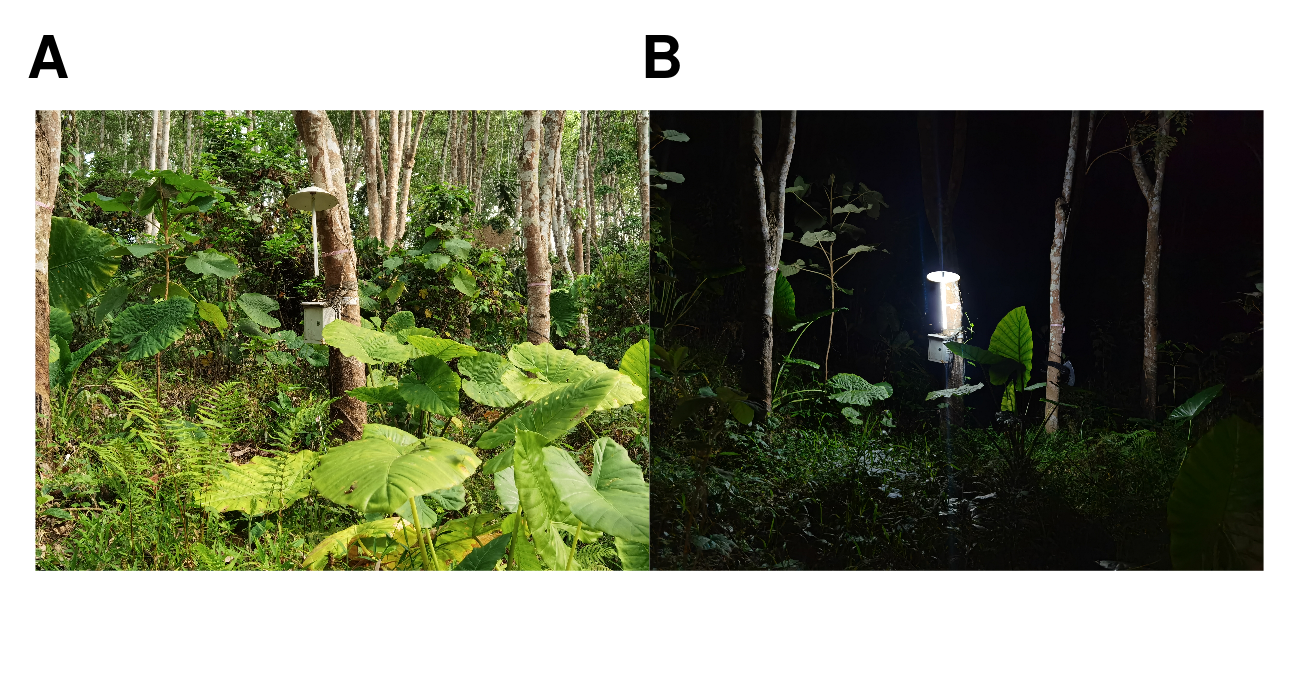
\includegraphics{/Users/mattocci/Dropbox/Reserach/MS/light_project/figs/merge.png}

}

\caption{\label{fig-alan}Photographs of the experimental setup during
daytime (A) and nighttime (B) in a rubber tree forest within the
Xishuangbanna Tropical Botanical Garden (XTBG), China.}

\end{figure}

\newpage

\begin{figure}

{\centering 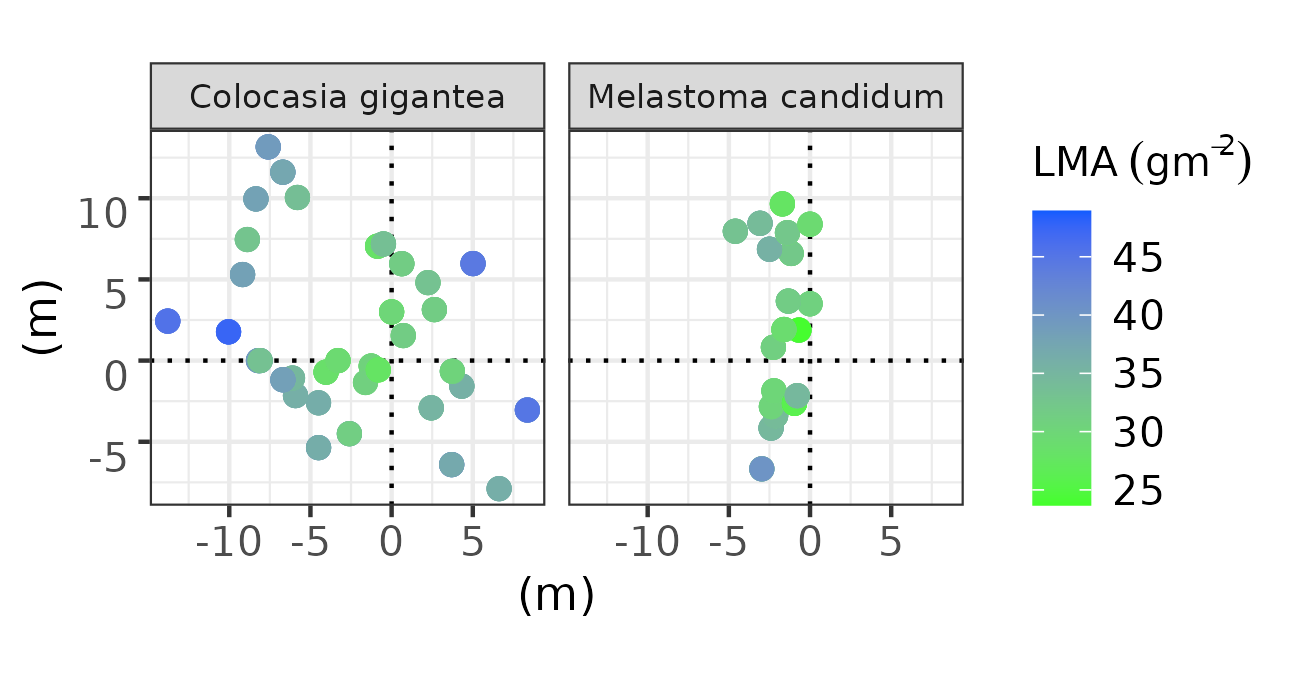
\includegraphics{/Users/mattocci/Dropbox/Reserach/MS/light_project/figs/lma_map.png}

}

\caption{\label{fig-LMA}Leaf mass per area (LMA) values of individuals
from the two experimental species, \emph{C. gigante} and \emph{M.
candidu}, in realtion to their relative geographic locations with
respect to the artificial light at night (ALAN). The ALANs are located
in the center of the maps (0, 0). Color represents the LMA values.}

\end{figure}

\newpage

\textbf{Table. 1.} Summary of Bayesian linear mixed-effect models
testing the effects of artificial light at night (ALAN), daylight, and
their interaction on leaf mass per area (LMA) values. Posterior means
and 95\% credible intervals (CI) are shown. Intervals that do not
include zero are highlighted in bold.

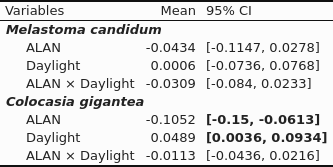
\includegraphics[width=3.125in,height=\textheight]{/Users/mattocci/Dropbox/Reserach/MS/light_project/figs/Table1.png}



\end{document}
